\subsection{Jeu mobile}
Le jeu mobile consiste en un jeu de rythme avec un écran divisé entre 4 zones verticales. Dans ces zones, des objectifs défilent du haut vers le bas et doivent être touchés par le joueur lorsqu'elles arrivent sur une ligne horizontale en bas de l'écran pour marquer des points.

\begin{figure}[h]
\begin{center}
\fbox{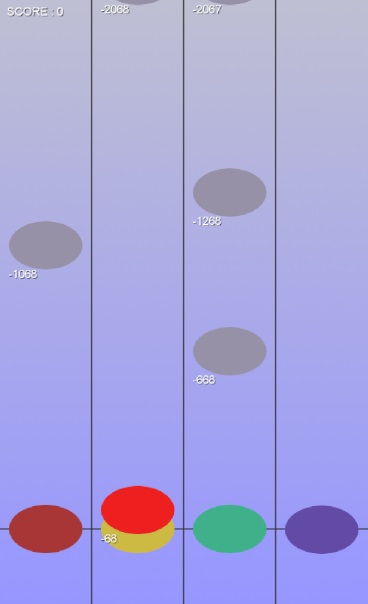
\includegraphics[scale=0.5]{images/jeu3.jpg}}
\end{center}
\caption{Jeu mobile}
\end{figure}

Un niveau se résume à une liste de zones (0,1,2,3) qui est associée à une liste d'instants.

Une fois le niveau lancé, le jeu se chargera d'afficher les objectifs aux bons endroits en tenant compte du temps écoulé depuis le début du niveau.

